\documentclass{beamer}

%% Fonts and encodings
\usepackage{multicol}
\usepackage{mathabx}
\usepackage[scaled]{helvet}
\usepackage{color}
\usepackage{lmodern}
\usepackage{eulervm}
\usepackage{wasysym}
\usefonttheme[onlymath]{serif}
\usefonttheme{professionalfonts}
\usefonttheme{structurebold}

\usepackage{bm}
\usepackage[utf8x]{inputenc}
\usepackage{booktabs}
\usepackage{natbib}
%% Color & Theme
\definecolor{SUblue}{RGB}{0,0,180}
\usecolortheme[RGB={0,0,180}]{structure}
\usetheme{Boadilla}
\setbeamertemplate{navigation symbols}{}
\setbeamertemplate{itemize items}[circle]
\setbeamertemplate{enumerate items}[circle]

\setbeamerfont{title}{size=\large}
\setbeamerfont{frametitle}{size=\normalsize}
\setbeamerfont{framesubtitle}{size=\small, shape =$\color{violet}{\looparrowdownright}~$}
\setbeamercolor{title}{fg=white, bg= SUblue!75!green}
\setbeamercolor{framesubtitle}{fg=violet}

\title[Dynamical Copula Modeling]{{\textbf{Dynamic Tail-Dependence and Correlation
      Modeling with Efficient Bayesian Approach}}}



\author[Feng Li]{\includegraphics[height=2cm]{cufelogo}\\
\vspace{0.5cm}\textbf{Feng Li}}
\institute[SAM.CUFE.EDU.CN]{\footnotesize{\textbf{School of Statistics and
      Mathematics\\ Central University of Finance and Economics}}}
\date{}

\begin{document}

% \begin{frame}[plain]
% \includegraphics[width=\textwidth]{FERM2014AD}
% \end{frame}


%% Title page
\begin{frame}[plain]
  \addtocounter{framenumber}{-1}
  \titlepage
\end{frame}

%% Outline
\section*{Outline}
\begin{frame}
  \frametitle{Outline}
  \addtocounter{framenumber}{-1}
  \tableofcontents
\end{frame}

%%%%%%%%%%%%%%%%%%%%%%%%%%%%%%%%%%%%%%%%%%%%%%%%%%%%%%%%%%%%%%%%%%%%%%%%%%%%%%%%
%% The main slides
%%%%%%%%%%%%%%%%%%%%%%%%%%%%%%%%%%%%%%%%%%%%%%%%%%%%%%%%%%%%%%%%%%%%%%%%%%%%%%%%

\section{A financial story}
 \begin{frame}
  \frametitle{The stock market returns for two indices}
    \begin{figure}
      \centering
      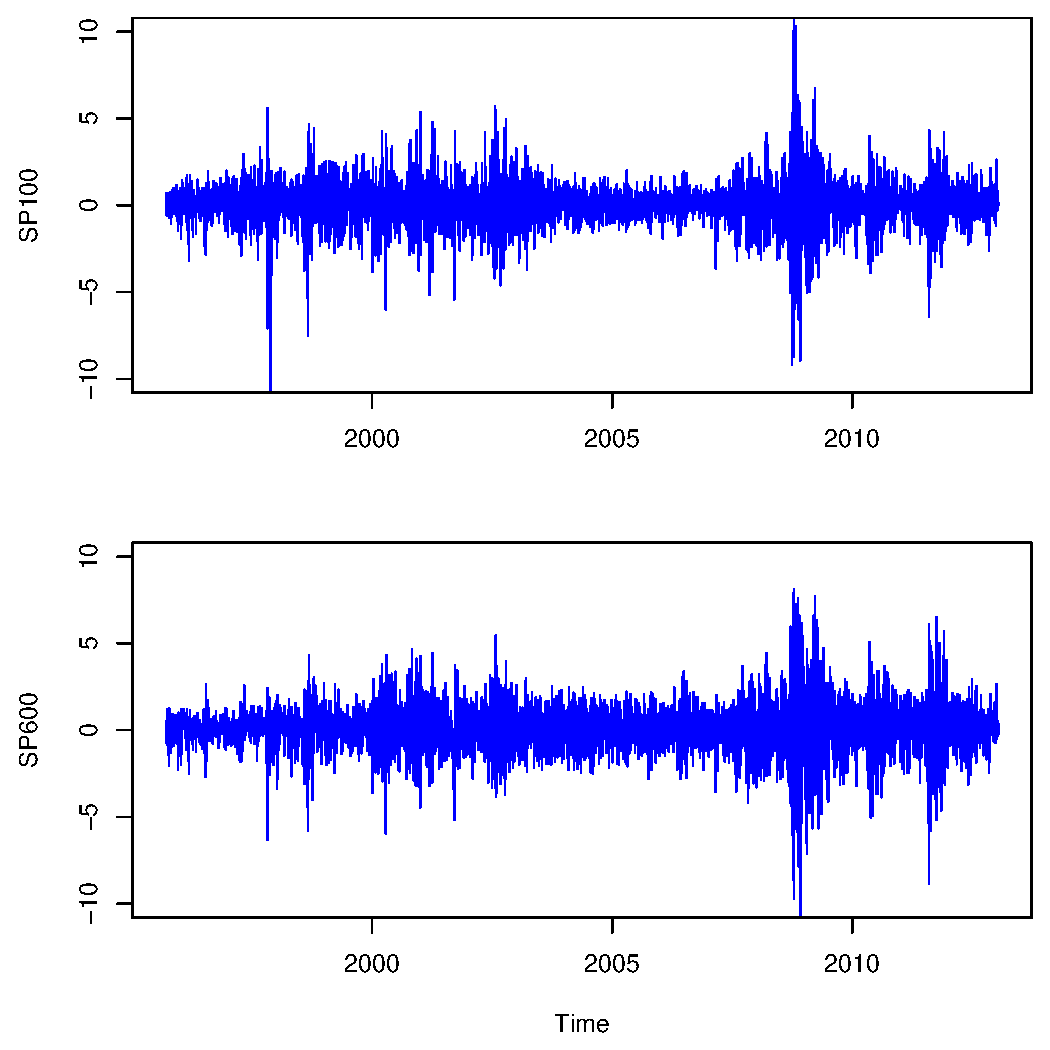
\includegraphics[height=0.9\textheight]{SP100-SP600}
    \end{figure}
\end{frame}

\begin{frame}
  \frametitle{Typical variables used in financial data}
  \begin{figure}
    \centering
    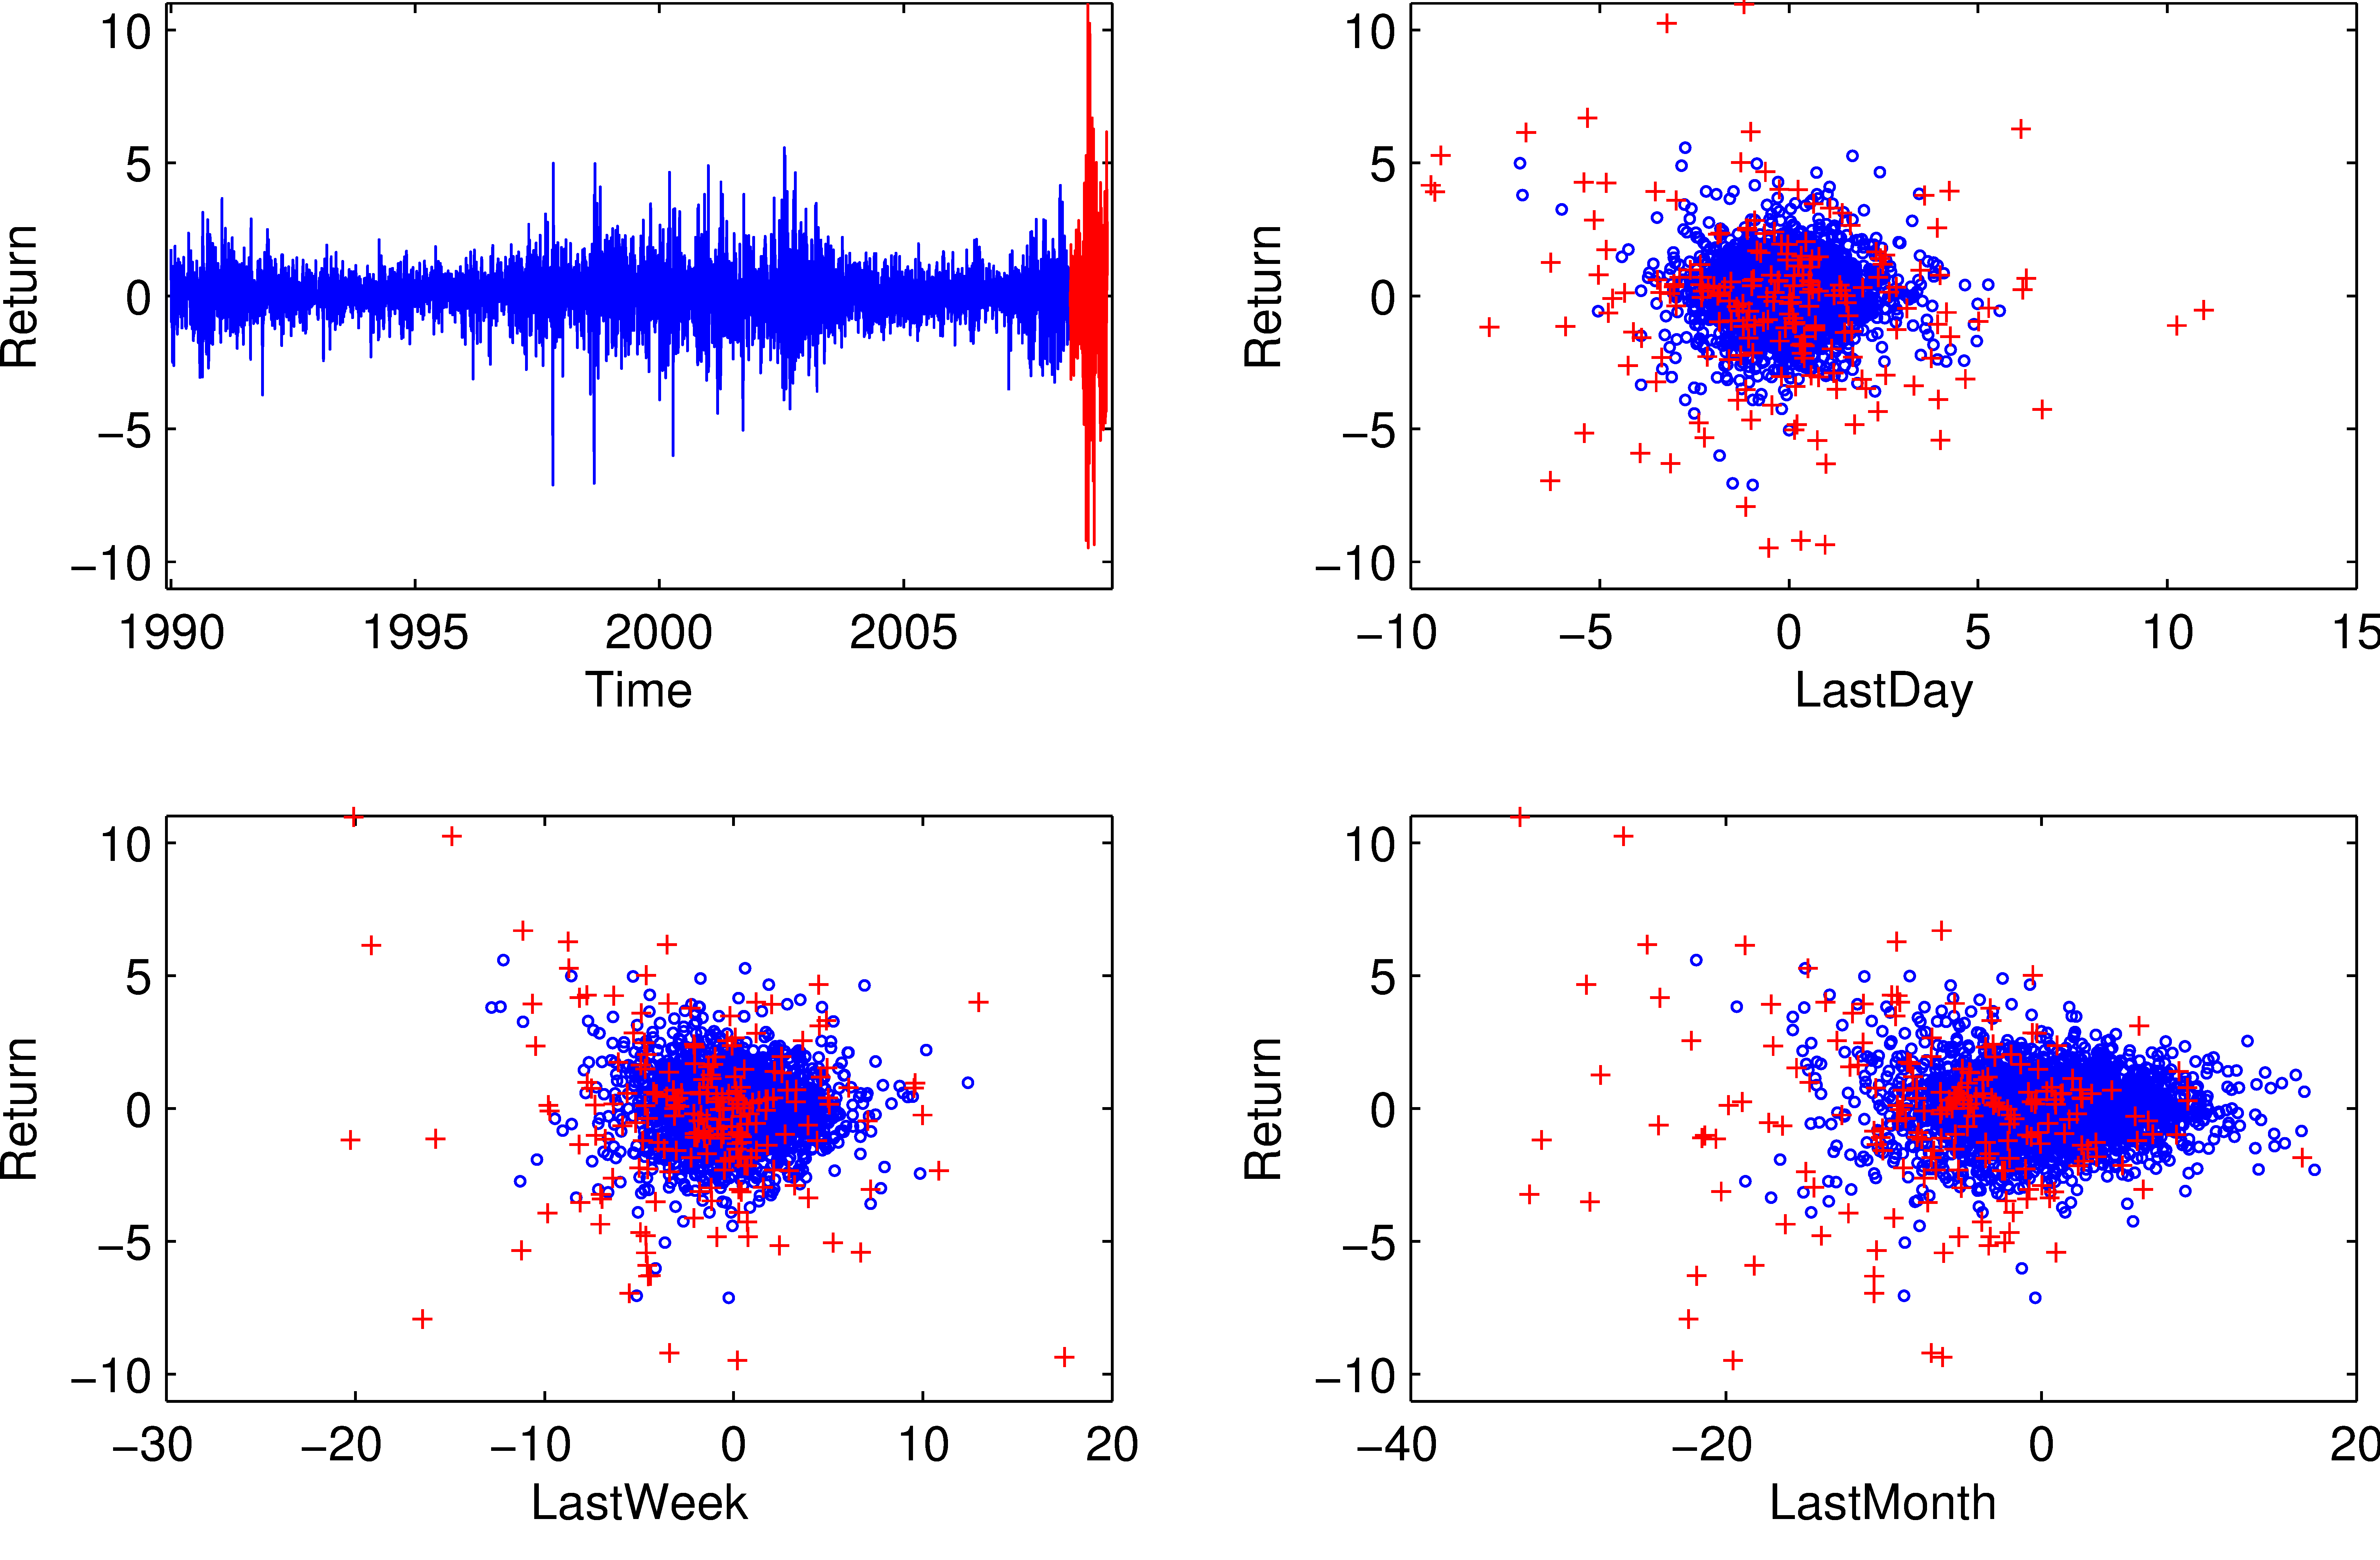
\includegraphics[height=0.8\textheight]{SP500}
  \end{figure}
\end{frame}


 \begin{frame}
  \frametitle{Individual Modeling the stock market returns}
    \begin{figure}
      \centering
      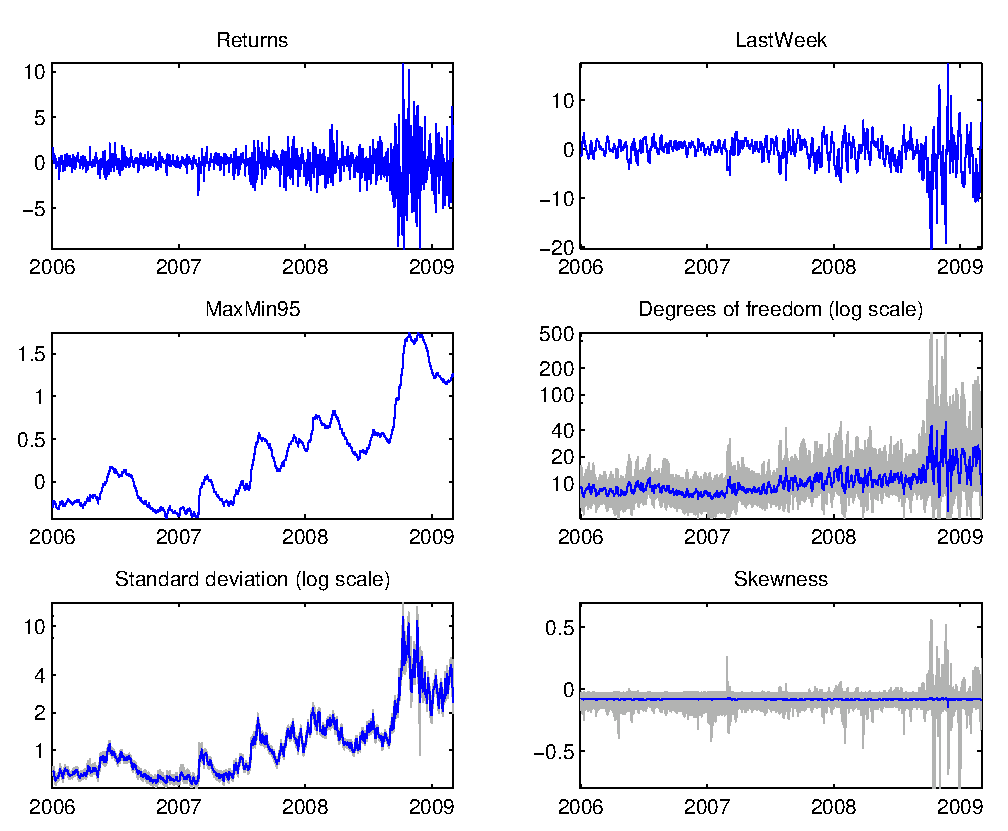
\includegraphics[height=0.9\textheight]{MomentPlotSP500}
    \end{figure}
\end{frame}

%\section{Introduction to copulas}
\begin{frame}
  \frametitle{Introduction to copulas}
  \framesubtitle{What is a copula?}
  \begin{itemize}
  \item The word ``copula'' means \textbf{linking}.
  \item \textbf{Sklar's theorem}

    Let $H$ be a multi-dimensional distribution function with marginal
    distribution functions $F_1(x_1),...,F_m(x_m)$. Then there exists a
    function $C$ (\textbf{copula function}) such that
    \begin{equation*}
      \begin{split}
        H(x_1,...,x_m)= & C(F_1(x_1),...,F_m(x_m))\\
        =&C\left(\int_{-\infty}^{x_1}f(z_1)dz_1,...,\int_{-\infty}^{x_m}f(z_m)dz_m\right)=C(u_1,...,u_m).
      \end{split}
    \end{equation*}
    Furthermore, if $F_i(x_i)$ are continuous, then $C$ is unique, and the derivative $c(u_1,...,u_m)= \partial^m C(u_1,...,u_m)/(\partial u_1...
    \partial u_m)$ is the \textbf{copula density}.

  \end{itemize}
\end{frame}


\section{Dynamical Measuring correlation and tail-dependence}
\begin{frame}
  \frametitle{Measuring correlation and tail dependence}
  \framesubtitle{Kendall's $\tau$ and tail-dependences}
  \begin{itemize}
  \item The \textbf{Kendall's $\tau$} can be written in terms of copula function:
    \begin{equation*}
      \begin{split}
        \tau = & 4 \int \int F(x_1, x_2)dF(x_1,x_2)-1 = 4 \int \int C(u_1, u_2)dC(u_1,u_2)-1. \\
      \end{split}
    \end{equation*}

  \item As well as the bivariate lower and upper \textbf{tail dependences}
    \begin{equation*}
      \begin{split}
        \lambda_L = & \lim \limits_{u \to 0^{+}} Pr(X_1< F_1^{-1}(u)| X_2<F_2^{-1}(u))= \lim \limits_{u \to 0^{+}} \frac{C(u,u)}{u},\\
        \lambda_U=&\lim \limits_{u \to 1^{-}} Pr(X_1> F_1^{-1}(u)|
        X_2>F_2^{-1}(u))= \lim \limits_{u \to 1^{-}} \frac{1-C(u,u)}{1-u}.\\
      \end{split}
    \end{equation*}

  \item Some facts:
    \begin{itemize}
    \item The Kendall's $\tau$ is invariant w.r.t. \textbf{strictly} increasing transformations.
    \item For all copulas in the elliptical class (Gaussian, \emph{t},...),
      $\tau = \frac{2}{\pi}arcsin(\rho)$.
    \item The Gaussian copula has zero tail dependence.
    \item The  student \texttt{t} copula has asymptotic upper tail dependence even for negative
      and zero correlations. The tail dependence decreases when degrees of
      freedom increases.
    \end{itemize}
  \end{itemize}
\end{frame}

\section{The covariate-contingent copula model}
\begin{frame}
  \frametitle{The covariate-contingent copula model}
  \framesubtitle{The Joe-Clayton copula}
  \begin{itemize}
  \item The Joe-Clayton copula function
    \[
    \begin{split}
      C(u,v,\theta,\delta)=&1-\left[1-\left\{\left(1-\bar u ^{\theta }\right)^{-\delta
          }+\left(1-\bar v ^{\theta }\right)^{-\delta }-1\right\}^{-1/\delta
        }\right]^{1/\theta }
    \end{split}
    \]
    where $\theta \geq 1$, $\delta > 0$, $\bar u = 1-u$, $\bar v = 1-v$ .

  \item Some properties:
    \begin{itemize}
    \item $\lambda_L=2^{-1/\delta}$ does not depend on $\lambda_U=2-2^{-1/\theta}$.
    \item  $\tau=1- 4\int _0^{\infty} s\times(\varphi'(s))^2ds$ is calculated via Laplace transform.
    \end{itemize}
  \end{itemize}

\end{frame}


\begin{frame}
  \frametitle{The covariate-contingent copula model}
  \framesubtitle{The reparameterized copula model}
  \begin{itemize}

  \item \textbf{The motivation}

    \begin{itemize}
    \item The interpretation of correlation and tail-dependence.
    \item Dynamical modeling tail-dependence and correlation.
    \end{itemize}

  \item \textbf{Reparametrization}: We reparameterize copula as a function of
    tail-dependence and Kendall's tau $C(\bm{u},\lambda_L, \lambda_L,\tau)$.
  \item \textbf{Applicable Copulas}: Any copula can be equally well used with such
    reparameterization.

    \begin{itemize}
    \item \textbf{Joe-Clayton Copula}: lower tail-dependence and upper tail-dependence are
      independent.
    \item \textbf{Gumbel Copula}: commonly used in extreme value theory.
    \item \textbf{Multivariate \emph{t} copula}: elliptical copula allows for
      tail-dependence with small df.
    \end{itemize}

  \end{itemize}
\end{frame}


\begin{frame}[plain]
  % \frametitle{The covariate-contingent copula model}
  % \framesubtitle{The dependence and correlation of Joe-Clayton copula}
  \begin{figure}
    \centering
    \vspace{-0.35cm}
    \includegraphics[width=0.46\textwidth]{BB7_tau-lamba.pdf}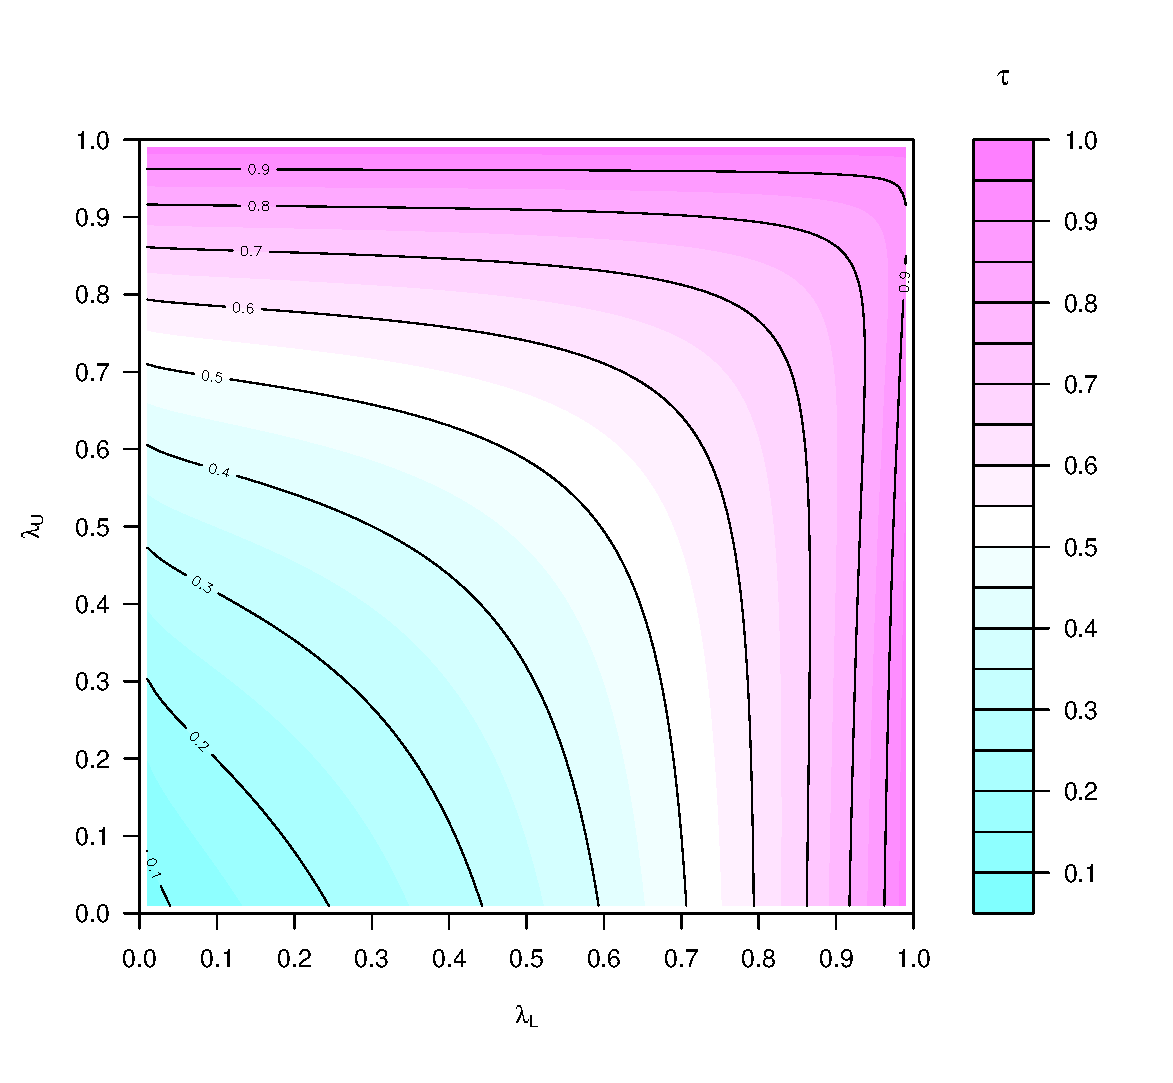
\includegraphics[width=0.56\textwidth]{tau-contour}\\
    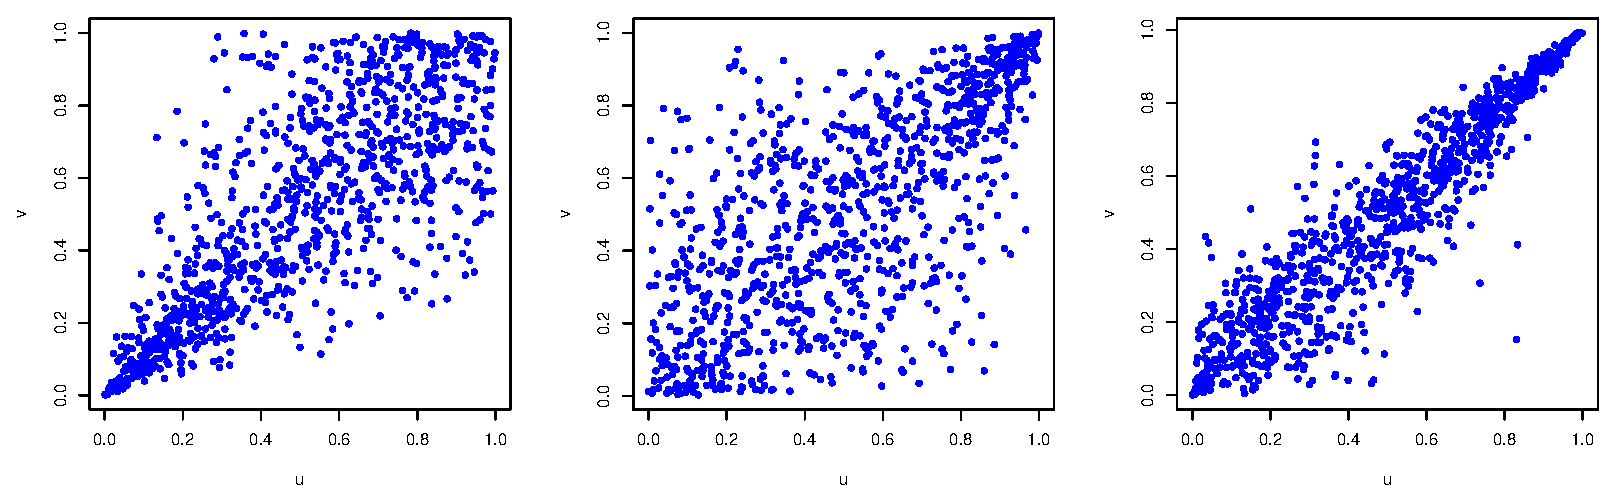
\includegraphics[width=\textwidth]{BB7Scatter.eps}
  \end{figure}
\end{frame}

\begin{frame}%[allowframebreaks]
  \frametitle{The covariate-contingent copula model}
  \framesubtitle{Connecting density features with covariates}

  \begin{itemize}
  \item All parameters are connected with covariates via known link function
    $\varphi(\cdot)$, (identity, log, logit, probit,...)
  \end{itemize}
    \begin{center}
      \begin{tabular}{lll}
        \toprule
      Components & Features & Linkage\\
        \midrule
        \small{Margins}&mean&$\mu = \varphi_{\beta_u}^{-1}(X_u\beta_u),$\\
                 &variance&$\sigma^2 = \varphi_{\beta_\sigma}^{-1}(X_\sigma\beta_\sigma),$ \\
                 &df&$\nu = \varphi_{\beta_\nu}^{-1}(X_\nu\beta_\nu),$\\
                 &skewness&$s = \varphi_{\beta_s}^{-1}(X_s\beta_s),$\\
%                 &...\\
        \small{Copula} &lower tail-dependence&$\lambda_L = \varphi_{\lambda}^{-1}((X_u,X_v)\beta_{\lambda_L}),$\\
                 &upper tail-dependence&$\lambda_U = \varphi_{\lambda}^{-1}((X_u,X_v)\beta_{\lambda_u}),$\\
                 &Kendall's $\tau$& $\tau=\varphi_{\tau}^{-1}((X_u,X_v)\beta_\tau).$\\
                 &Covariance Matrix\color{blue}{*}& $\Sigma=\Sigma_0 + \kappa I$ where\\
                 &&\hspace{0.4cm}$\mathrm{vech}(\bm{\Sigma_0}) = \varphi^{-1}([\bm{I}\otimes \bm{X}]\mathrm{vec}\bm{B})$\\
        \bottomrule
      \end{tabular}
      \begin{itemize}
      \item [*] \small{Cholesky decomposition {\color{blue}\citep{huang2007estimation}} is
          possible but not interpretation friendly.}
      \end{itemize}
    \end{center}


      \begin{align*}
      \end{align*}

    \end{frame}

\begin{frame}[allowframebreaks]
\frametitle{The covariate-contingent copula model}
\framesubtitle{The Bayesian approach}
\begin{itemize}
\item \textbf{The marginal models}
    \begin{itemize}
    \item In principle, any combination of univariate marginal models can be
      used.
    \item When there are discrete margins, data augmentation method can be used
      {\color{blue}\citep{smith2012estimation}}.

    \item We develop R package to allow for
      \begin{itemize}
      \item mixtures of elliptical distributions {\color{blue}\citep{li2010flexible}}
      \item regression spline where the knots locations are treated as unknown parameters
        {\color{blue}\citep{li2013efficient}}.
      \end{itemize}


    \item In the continuous case, we use univariate model that each margin is
      from the student \emph{t} distribution \color{blue}{\citep{li2010flexible}}.
    \end{itemize}

  \item \textbf{The log Posterior}
\[
\begin{split}\log p(\{\bm{\beta},\bm{\mathcal{I}}\}|\bm{y},\bm{x})=
  \mathrm{c}&+\sum\nolimits _{j=1}^{M}\left\{\log
  p(\bm{y}_{.j}|\{\bm{\beta},\bm{\mathcal{I}}\}_{j},\bm{x}_{j}) + \log p(\{\bm{\beta},\bm{\mathcal{I}}_j\}) \right\}\\
 & +\log\mathcal{L}_{C}(\bm{u}_{1:M}|\{\bm{\beta},\bm{\mathcal{I}}\}_{C},\bm{y},\bm{x})+
 \log p_C(\{\bm{\beta},\bm{\mathcal{I}}\})
\end{split}
\]

where
\begin{itemize}
\item $\{\bm{\beta}\}$ are the coefficient in the linking function,
\item $\{\bm{\mathcal{I}}\}$ are the corresponding variable selection indicators.
\item $\{\bm{\beta},\bm{\mathcal{I}}\}$ can be estimated jointly via Bayesian approach.
\item $\bm{u}_{j}=F_{j}(y_{j})$ is the CDF of the $j$:th marginal model.
\end{itemize}

    % \begin{equation*}
    %   \begin{split}
    %     & \log \mathcal{L} (Y_u,Y_v| X_u, X_v,\lambda_L, \tau,\beta_u,\beta_v) =  \sum_{i=1}^{n}
    %     \log c(u_i,v_i, \lambda_L, \tau) \\
    %     & \hspace{2.8cm}  + \log \mathcal{L}_u(Y_u|X_u,\beta_u) + \log \mathcal{L}_v(Y_v|X_v,\beta_v)\\
    %   \end{split}
    % \end{equation*}

  \end{itemize}
\end{frame}

\section{The Bayesian Scheme}

\begin{frame}
  \frametitle{The covariate-contingent copula model}
  \framesubtitle{The Bayesian approach}
  \begin{itemize}

  \item \textbf{The priors} for the copula model are easy to specify due to our
    reparameterization.

    \begin{itemize}

    \item It it \textbf{not easy} to specify priors directly on
      $\{\bm{\beta},\bm{\mathcal{I}}\}$

    \item But it is \textbf{easy} to puts prior information on the model parameters
      features ($\tau$, $\mu$, $\sigma^2$) and then derive the implied prior on the
      intercepts and variable selection indicators.

    \item When variable selection is used, we assume there are no covariates in
      the link functions \emph{a priori}.

    \end{itemize}

  \item \textbf{The posterior} inference is straightforward although the model is very
    complicated.
  \end{itemize}
\end{frame}

\begin{frame}[allowframebreaks]
  \frametitle{The dynamic copula model}
  \framesubtitle{Sampling the posterior with an efficient MCMC scheme}
  \begin{itemize}
  \item We update all the parameters \textbf{jointly} by using tailored
    Metropolis-Hastings within Gibbs.
  \item The proposal density for each parameter vector $\beta$ is a multivariate \emph{t}-density with  $df>2$,
    \[
    \bm{\beta}_{p} |\bm{\beta}_{c}\sim\bm{MVT}\left[\bm{\hat{\beta}},~\left.-\left(\frac{\partial^{2}\ln
            p(\bm{\beta}|\bm{Y})}{\partial\bm{\beta}\partial\bm{\beta}^{\prime}}\right)^{-1}\right\vert
      _{\bm{\beta}=\bm{\hat{\beta}}},~df\right],
    \]
    where $\bm{\hat{\beta}}$ is obtained by $R$ steps ($R\leq 3$) Newton's
    iterations during the proposal with analytical gradients.

  \item This approach has some flavor of Hamiltonian MC when $R=1$ (Thanks Rong Chen for
    pointing this out).

  \item \textbf{Bayesian variable selection} is carried out simultaneously.

  % \item It is eventually straightforward. Thanks to the chain rule!

  \end{itemize}


  \begin{itemize}
  \item The Gibbs sampler for covariate-dependent copula.
  \item The notation $\{\beta_{\mu},\mathcal{I}_{\mu}\}_{-m}$ indicates all other
    parameters in the model except $\{\beta_{\mu},\mathcal{I}_{\mu}\}_{m}$. The updating
    order is column-wise from left to right. If dependent link functions are used, the
    updating should be ordered accordingly.
  \end{itemize}
\begin{table}
  \label{tab:gibbs}
  \centering
  \resizebox{\textwidth}{!}{
    \begin{tabular}{llll}
      \toprule
      Margin component $(1)$ & ...  & Margin component ($M$) & Copula component ($C$)\tabularnewline
      \midrule
      $(1.1)$ $\{\beta_{\mu},\mathcal{I}_{\mu}\}_{1}|\{\beta_{\mu},\mathcal{I}_{\mu}\}_{-1}$  & ...  & $(M.1)$ $\{\beta_{\mu},\mathcal{I}_{\mu}\}_{M}|\{\beta_{\mu},\mathcal{I}_{\mu}\}_{-M}$  & $(C.1)$ $\{\beta_{\lambda},\mathcal{I}_{\lambda}\}_{C}|\{\beta_{\lambda},\mathcal{I}_{\lambda}\}_{-C}$\tabularnewline
      $(1.2)$ $\{\beta_{\phi},\mathcal{I}_{\phi}\}_{1}|\{\beta_{\phi},\mathcal{I}_{\phi}\}_{-1}$  & ...  & $(M.2)$ $\{\beta_{\phi},\mathcal{I}_{\phi}\}_{M}|\{\beta_{\phi},\mathcal{I}_{\phi}\}_{-M}$  & $(C.2)$ $\{\beta_{\tau},\mathcal{I}_{\tau}\}_{C}|\{\beta_{\tau},\mathcal{I}_{\tau}\}_{-C}$\tabularnewline
      $(1.3)$ $\{\beta_{\nu},\mathcal{I}_{\nu}\}_{1}|\{\beta_{\nu},\mathcal{I}_{\nu}\}_{-1}$  & ...  & $(M.3)$ $\{\beta_{\nu},\mathcal{I}_{\nu}\}_{M}|\{\beta_{\nu},\mathcal{I}_{\nu}\}_{-M}$  & \tabularnewline
      $(1.4)$ $\{\beta_{\kappa},\mathcal{I}_{\kappa}\}_{1}|\{\beta_{\kappa},\mathcal{I}_{\kappa}\}_{-1}$  & ...  & $(M.4)$ $\{\beta_{\kappa},\mathcal{I}_{\kappa}\}_{M}|\{\beta_{\kappa},\mathcal{I}_{\kappa}\}_{-M}$  & \tabularnewline
      \bottomrule
    \end{tabular}
  }
\end{table}

\end{frame}

\begin{frame}[allowframebreaks]
  \frametitle{The dynamic copula model}
  \framesubtitle{The computational details}
  \begin{itemize}

  \item \textbf{Taming the Beast:} the analytical gradients require the derivative for the
    copula density and marginal densities which can be conveniently decomposed via the
    chain rule that greatly reduces the complexity of the the gradient calculation.
    {\footnotesize
      \begin{align*}
        \frac{\partial\log c(u_{1:M},\lambda_{L},\tau)}{\partial\lambda_{L}}= & \frac{\partial\log c(u_{1:M},\theta,\delta)}{\partial\delta}\times\left(\frac{\partial\lambda_{L}}{\partial\delta}\right)^{-1}\\
                                                                              &+\frac{\partial\log c(u_{1:M},\theta,\delta)}{\partial\theta}\times\left(\frac{\partial\lambda_{L}}{\partial\theta}\right)^{-1}\\
        \frac{\partial\log c(u_{1:M},\lambda_{L},\tau)}{\partial\tau}= &
                                                                         \frac{\partial\log c(u_{1:M},\theta,\delta)}{\partial\theta}\times\left(\frac{\partial\tau(\theta,\delta)}{\partial\theta}\right)^{-1}\\
                                                                              & +                                                                           \frac{\partial\log c(u_{1:M},\theta,\delta)}{\partial\delta}\times\left(\frac{\partial\tau(\theta,\delta)}{\partial\delta}\right)^{-1}\\
        \frac{\partial\log c(u_{1:M},,\lambda_{L},\tau)}{\partial\varphi_{m}}= &
                                                                                 \frac{\partial\log c(u_{1:M},,\theta,\delta)}{\partial u_{m}}\times\frac{\partial
                                                                                 u_{m}}{\partial\varphi_m}\\ &+ \frac{\partial \log
                                                                                                               p_m(y_m,\varphi_m)}{\partial \varphi_m}
      \end{align*}
    }

  \item The direct derivatives of CDF function and PDF functions with respect to their
    parameters are straightforward for most densities.

  \item Existing derivatives for PDF functions in marginal models:

    \begin{itemize}
    \item {\color{blue}\citet{li2010flexible}} (mixtures of asymmetric student-\emph{t}
      densities where asymmetric normal and symmetric student-\emph{t} densities are its
      special cases),

    \item {\color{blue}\citet{li2011modeling}} (gamma and log-normal models)
  \item {\color{blue}\citet{villani2012generalized}} (negative binomial, beta and
    generalized Poisson models)
  \item {\color{blue}\citet{li2013efficient}} (spline model with knots location as unknown
    parameters).  densities)
    \end{itemize}

  \item {\color{blue}{Li (2015, JBES forthcoming)}} (derivatives for Joe-Clayton copula,
    Gumbel copula and  multivariate \emph{t} copula).

  \item \textbf{The bad news}: Evaluating the gradients are very time consuming if we do
    it sequentially, e.g.

    \begin{itemize}
    \item when t copula is used, the tail-dependence for $i$th and $j$th margins
      ($\lambda_{Lij}$) are {\color{blue}\citep{embrechts1997modelling}}
    \begin{align*}
      \lambda_{Lij} = \frac{\int _{\pi/4 - \mathrm{arcsin}
      (\rho_{ij})/2}^{\pi/2}\mathrm{cos}^{\nu}(t)dt}{\int _0^{\pi} \mathrm{cos}^{\nu} (t) d t}
    \end{align*}
    and $\rho_{ij}$ is the correlation coefficient for $i$th and $j$th margins.

  \item Kendall's $\tau$ of the Joe-Clayton copula is of the form
\[
\tau(\theta,\delta)=\begin{cases}
1-2/[\delta(2-\theta)]+4B\left(\delta+2,2/\theta-1\right)/(\theta^{2}\delta), &{\hspace{-2cm}}1\leq\theta<2;\\
1-\left[\psi(2+\delta)-\psi(1)-1\right]/\delta, &{\hspace{-2cm}} \theta=2;\\
1-2/[\delta(2-\theta)]&{\hspace{-2cm}}\theta>2\\{\hspace{0.3cm}}-4\pi/\left[\theta^{2}\delta(2+\delta)\sin(2\pi/\theta)B\left(1+\delta+2/\theta,2-2/\theta\right)\right], &
\end{cases}
\]

    \end{itemize}

  \item \textbf{The good news}: the gradient can be evaluated parallelly because we assume
    the observations are independent.

  \item Our parallel version code running on a 16-core CPU can speed up the
    computation at least \textbf{10X}.

  \item The code is running on a cluster with 80 cores and total 1TB RAM.

  \item \textbf{Why not random walk Metropolis or RJMCMC}?

    \begin{itemize}
    \item Random walk Metropolis or RJMCMC are very inefficient in such complicated model.
    \item Our tailored Metropolis-Hastings will obtain the overall acceptance probability
      \textbf{80\%}.
    \item The efficiency speed up is about \textbf{50X}.
    \end{itemize}

\newpage
  \item \textbf{Why not two-stage approach}?

    \begin{itemize}
    \item The asymptotic relative efficiency of the two-stage estimation procedure depends
      on how close the copula is to the Fr\'echet bounds
      {\color{blue}\citep{joe2005asymptotic}}.
    \item The two-stage approach in estimating the multivariate DCC GARCH model is
      consistent but not fully efficient due to the limited information provided by the
      estimators {\color{blue}\citep{engle2001theoretical}}.

    \end{itemize}

  \end{itemize}
\end{frame}

\begin{frame}
\frametitle{Model Comparison}
  \begin{itemize}
  \item We evaluating the model performance based on \textbf{out-of-sample prediction}.
  \item In our time series application, we estimate the model based on the 80\% of
    historical data and then predict the last 20\% data.

  \item We evaluate the quality of the one-step-ahead predictions using the \textbf{log
      predictive score} (LPS)
\begin{align*}
\mathrm{LPS}=&\log p(D_{(T+1):(T+p)}|D_{1:T})\\
               =&\sum\nolimits _{i=1}^{p}\log\int p(D_{T+i}|\theta,D_{1:(T+i-1)})p(\theta|D_{1:(T+i-1)})\mathrm{d}\theta
\end{align*}
where $D_{a:b}$ is the dataset from time $a$ to $b$ and $\theta$ are the model
parameters.
  \end{itemize}
\end{frame}


\section{Empirical study and extensions}

\begin{frame}[plain]
  \addtocounter{framenumber}{-1}

  \begin{center}
    {\Large \color{blue}{\textbf{The stock returns, a revisit}}}
  \end{center}
\end{frame}

\begin{frame}
  \frametitle{The Kendall's $\tau$ (left column) and tail-dependence (right column) over
    time for SP100 (top row) and SP600 (bottom row)}
  \begin{figure}
    \centering
    \hspace{-1cm}
\includegraphics[height=0.4\textheight]{var-post}\\
    \hspace{-1cm}
\includegraphics[height=0.41\textheight]{tau-post}
  \end{figure}
\end{frame}


\begin{frame}
  \frametitle{The posterior copula plot}
  \begin{figure}
    \centering
    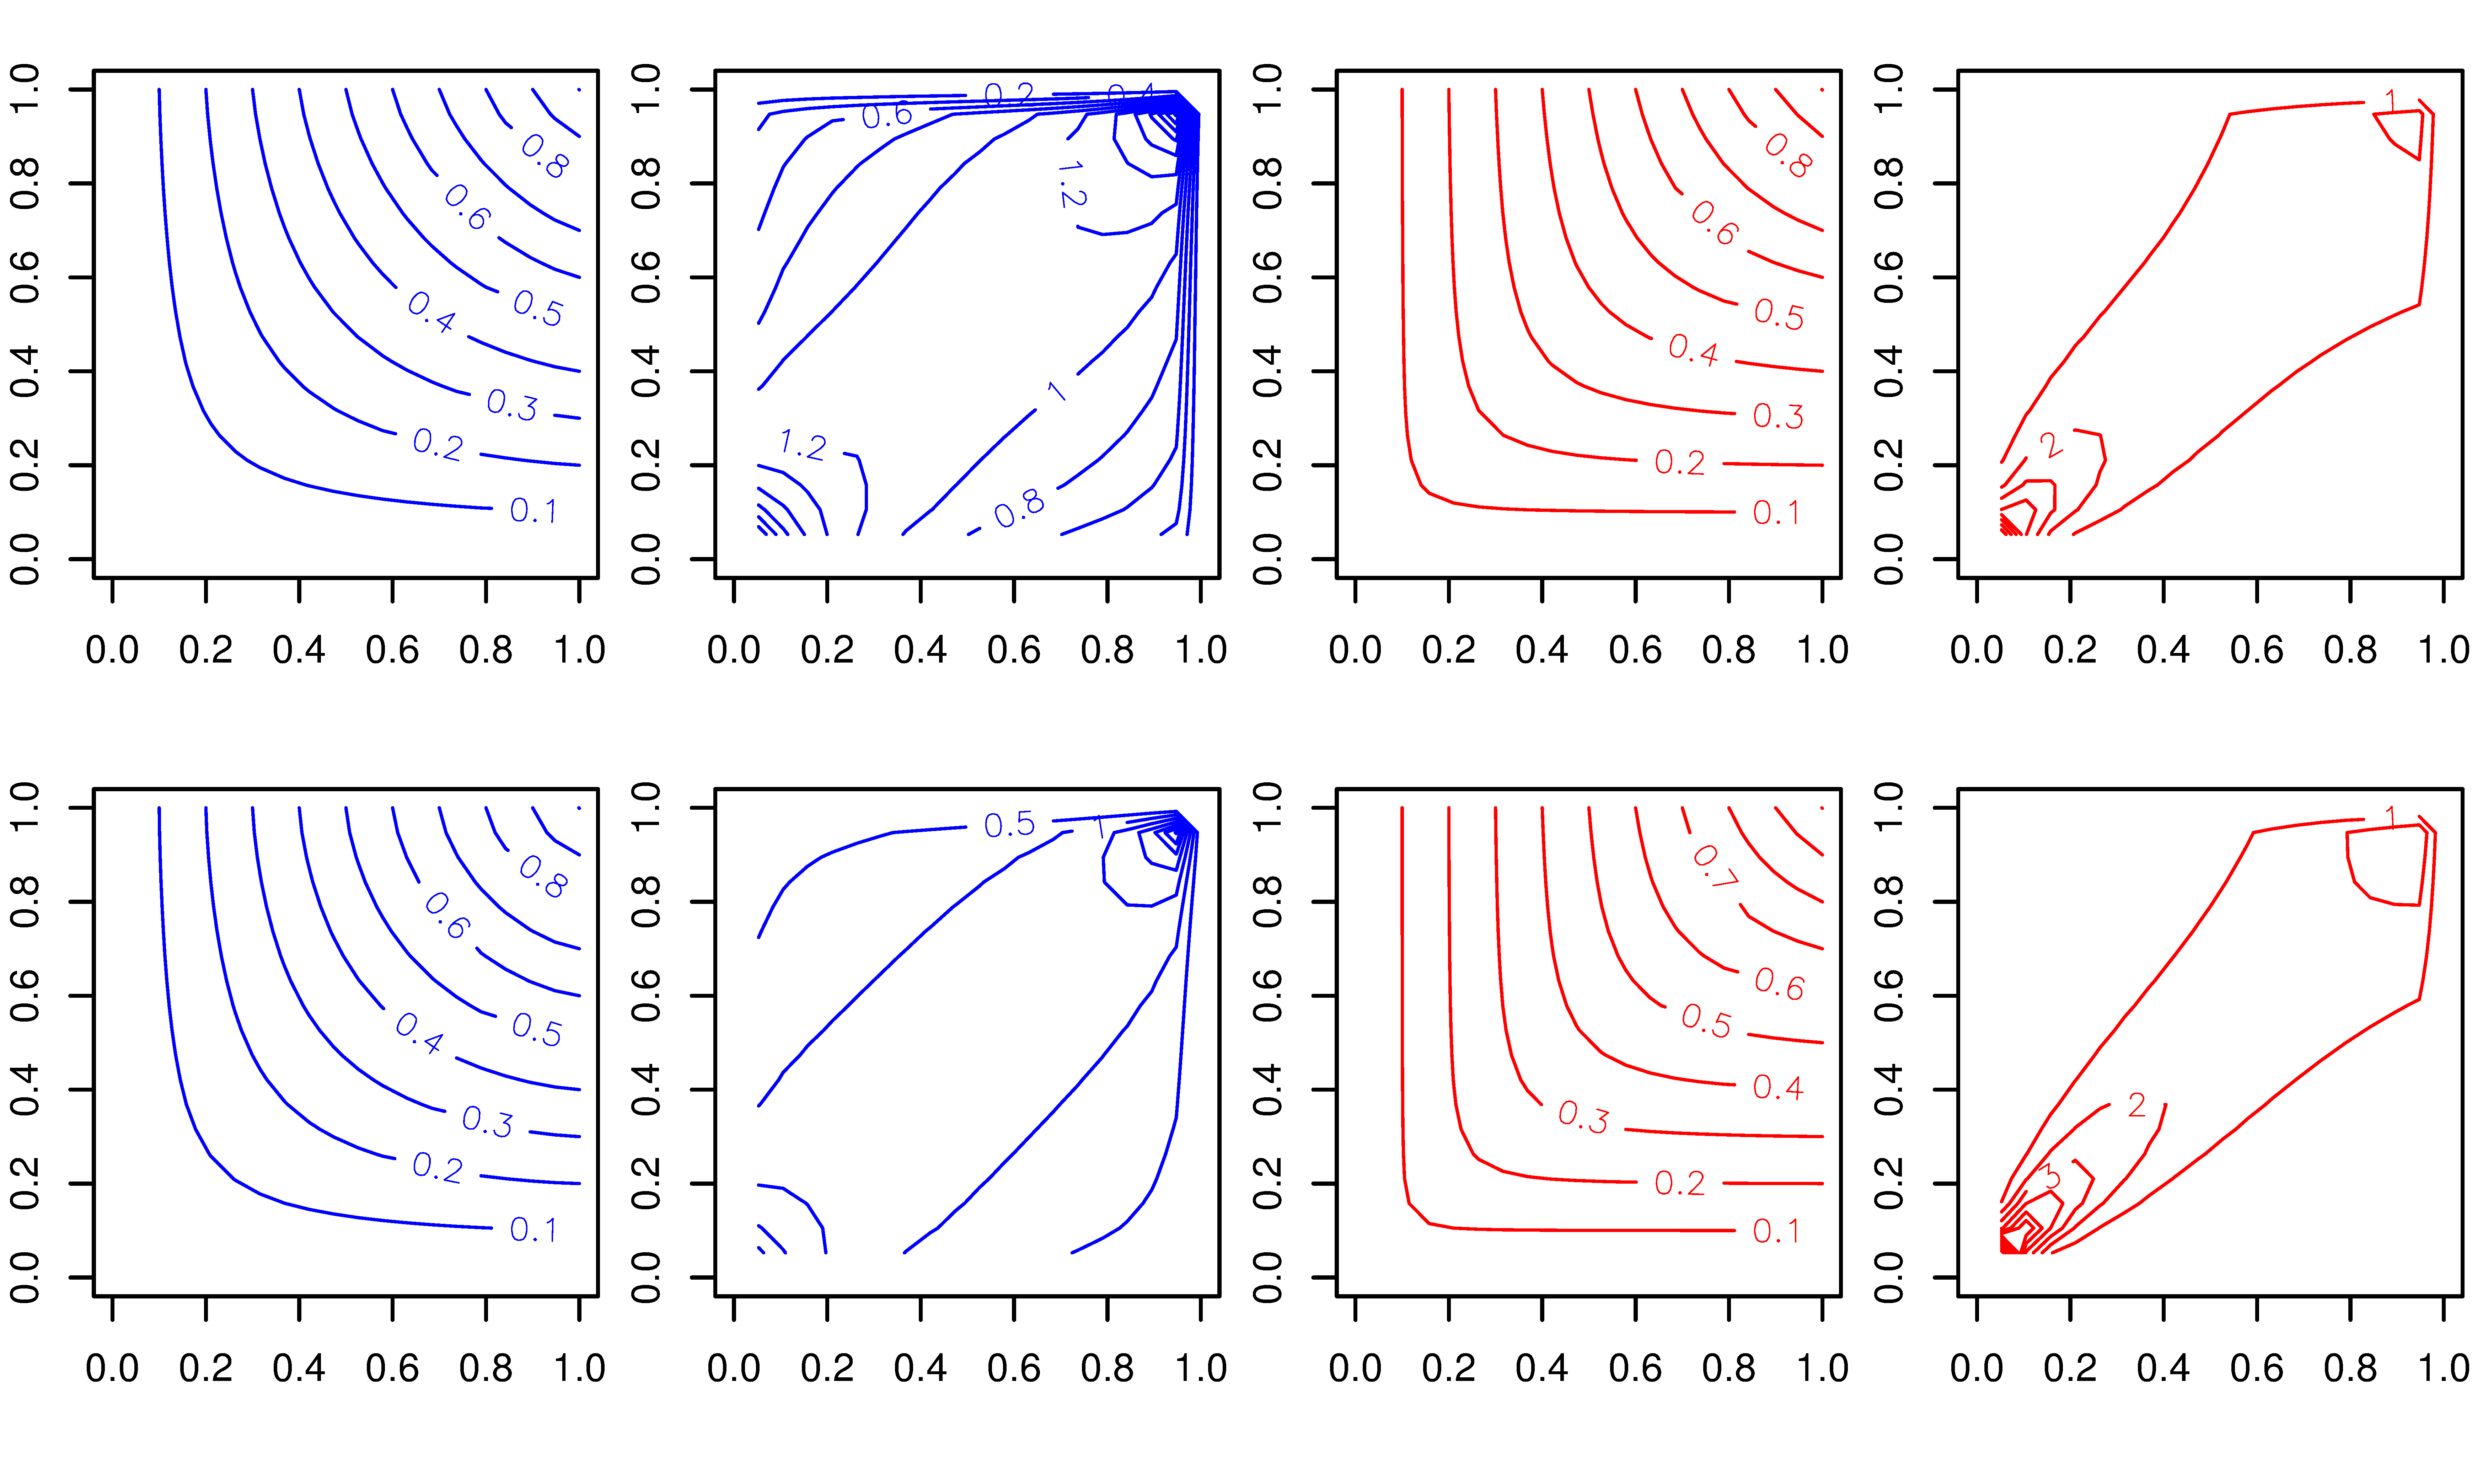
\includegraphics[height=0.8\textheight]{contour}
  \end{figure}
\end{frame}


\begin{frame}
\begin{table}
  \caption{Posterior summary of copula model with S\&P100 and S\&P600 data. In
    the copula component part, the first row and second row for $\beta$ and $\mathcal{I}$ are the results for the
    combined covariates that are used in the first and second marginal model,
    respectively. The intercept are always included in the model.}
  \label{tab:sp-fullrun}
  \centering
  \resizebox{\columnwidth}{!}{%
    \begin{tabular}{rrrrrrrrrrr}
    \toprule
    &\textsf{Intercept}&\textsf{RM1}&\textsf{RM5}&\textsf{RM20}
    &\textsf{CloseAbs95}& \textsf{CloseAbs80}& \textsf{MaxMin95}
    & \textsf{MaxMin80}&\textsf{CloseSqr95}& \textsf{CloseSqr80}\\

    \cmidrule(r){2-11}
\vspace{0.1cm}\\
\multicolumn{11}{c}{Copula component ($C$)}\\
\vspace{0.05cm}\\

$\beta_{\lambda_L}$&$-8.165$&$\mathbf{-0.555}$&$1.793$&$\mathbf{0.005}$&$-0.170$&$\mathbf{0.110}$&$-0.667$&$-1.448$&$-0.636$&$0.050$\\
               &&$\mathbf{1.463}$&$\mathbf{0.405}$&$0.934$&$-2.138$&$-1.288$&$-1.954$&$-1.577$&$\mathbf{-1.873}$&$-1.805$\\
\\
$\mathcal{I}_{\lambda_L}$&$1.00$&$\mathbf{0.98}$&$0.37$&$\mathbf{0.63}$&$0.02$&$\mathbf{0.61}$&$0.36$&$0.35$&$0.39$&$0.29$\\
                    &&$\mathbf{1.00}$& $\mathbf{1.00}$&$0.00$&$0.30$&$0.35$&$0.40$&$0.00$&$\mathbf{0.61}$&$0.34$\\

&\\

$\beta_{\tau}$&$-1.726$&$0.181$&$-0.217$&$-0.304$&$-0.107$&$\mathbf{0.115}$&$\mathbf{0.005}$&$\mathbf{-0.257}$&$\mathbf{1.068}$&$0.037$\\
             && $\mathbf{-0.191}$&$\mathbf{0.170}$&$0.274$&$0.144$&$\mathbf{-0.051}$&$\mathbf{-0.671}$&$0.059$&$-0.209$&$-0.181$\\
\\
$\mathcal{I}_{\tau}$& $1.00$&$0.00$&$0.00$&$0.00$&$0.00$&$\mathbf{0.90}$&$\mathbf{0.99}$&$\mathbf{1.00}$&$\mathbf{0.85}$&$0.00$\\
                  & &$\mathbf{1.00}$&$\mathbf{1.00}$&$0.00$&$0.00$&$\mathbf{1.00}$&$\mathbf{1.00}$&$0.00$&$0.00$&$0.00$\\


\bottomrule
  \end{tabular}
}
\flushleft \footnotesize{The inefficiency factors for the parameters are all bellow $25$.}
\end{table}
\end{frame}

\begin{frame}
  \frametitle{Extensions and future work}
  \begin{enumerate}
  \item We are working to extend the model in text mining and financial modeling that
    allow some margins are continuous but some are discrete.

    \begin{itemize}
    \item One margin: A company's stock credited as $A$, $A^+$ over time by
      Standard \& Poor's.
    \item The other margin: the stock returns over time
    \end{itemize}

  \item Efficient approximation of the posterior via sub-sampling to handle much bigger
    data. Several Big Data MCMC approaches have been already considered in
    {\color{blue}Welling and Teh (2011), Korattikara et al. (2013), Teh et al. (2014),
      Bardenet et al. (2014), Maclaurin and Adams (2014), Minsker et al.  (2014), Quiroz
      et al. (2014)} and {\color{blue}Strathmann et al. (2015)} but not in such general
    model.

  \end{enumerate}
\end{frame}

\begin{frame}[allowframebreaks]
  \frametitle{References}
  \bibliography{References,full}
  \bibliographystyle{asa}
\end{frame}

\begin{frame}[plain]
  \addtocounter{framenumber}{-1}
  \begin{center}
    {\color{SUblue} \textbf{\Huge Thank you!}}
    \vspace{1cm}

    {\texttt{\textbf{\url{feng.li@cufe.edu.cn}}}}

    \vspace{1cm}

    {\texttt{\textbf{\url{http://feng.li/}}}}

  \end{center}
\end{frame}

\end{document}
